\chapter{MapReduce}
\label{chap:mapreduce}

Instances of MapReduce are Hadoop and Spark. We will discuss them later.
As stated in \autoref{chap:big_data}, Google was a pioneer in Big Data processing, and introduced the MapReduce framework in 2004.

Distributed computing is the key to Big Data processing, as it allows to \textit{split} huge tasks into smaller ones, \textit{parallely} execute, and \textit{aggregate} the results to provide a final output.\\
This is also known in data-analysis as \textit{split-apply-combine}.

\section{MapReduce Framework}

\begin{paracol}{2}
   \begin{center}
      \texttt{Map}\\
      $Map(key_a), value_1) \rightarrow list(key_b, value_2)$
   \end{center}
   Various kind of processing on the input data may be done, typically filtering and sorting.
   \note{Note how the signature is slightly different from the typical map}
   \switchcolumn
   \begin{center}
      \texttt{Reduce}\\
      $Reduce(key_b, list(value_2)) \rightarrow list((key_c,value_3))$
   \end{center}
   \texttt{Reduce} refers to the summarization, produced in an associative way, of the results produced by \lstinline|Map|.
   \note{Each Reduce call typically produces either one key value pair or an empty return, though one call is allowed to return more than one key value pair.}
\end{paracol}

\begin{enumerate}
   \item \textbf{Map} - Each worker node applies the \lstinline|Map| function to the local data, and writes the output to a temporary storage.
   \item \textbf{Shuffle} - worker nodes redistribute data based on the output keys, such that all data belonging to one key is located on the same worker node.
   \item \textbf{Reduce} - worker nodes now process each group of output data, per key, in parallel.
\end{enumerate}

\begin{figure}[htbp]
   \centering
   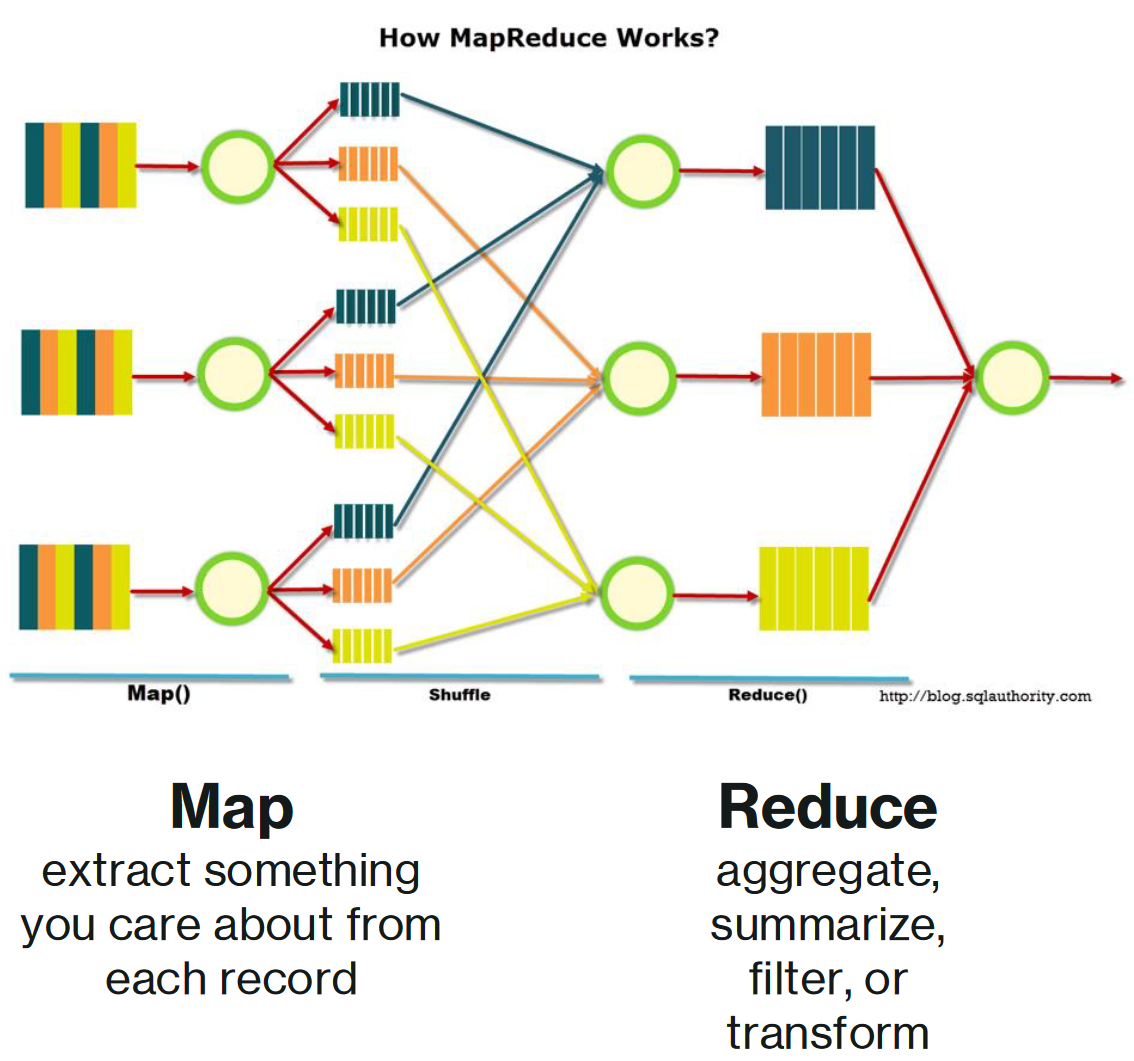
\includegraphics[width=0.4\columnwidth]{images/14/mapreduce_overview.png}
   \caption{MapReduce overview}
   \label{fig:14/mapreduce_overview}
\end{figure}


\newpage
\section{Instatiating MapReduce}
\begin{figure}[htbp]
   \centering
   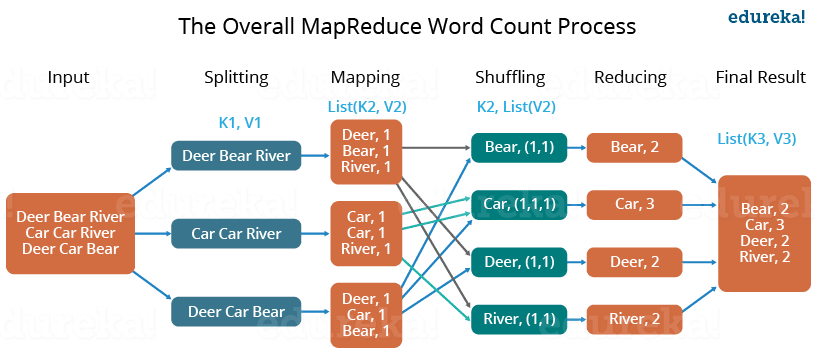
\includegraphics{images/14/mapreduce_wordcount.png}
   \caption{MapReduce WordCount example}
   \label{fig:14/mapreduce_wordcount}
\end{figure}

\begin{itemize}
   \item One \texttt{JobTracker} to which client applications
   submit MapReduce jobs
   \item JobTracker pushes work to available \texttt{TaskTracker} nodes in the cluster keeping the work close to the data
   \item With a \textbf{rack-aware} file system the \texttt{JobTracker} knows which node contains the data.
   \note{If the work cannot be hosted on the actual node where the data resides, priority is given to nodes in the same rack}
\end{itemize}

If a \texttt{TaskTracker} fails or times out, that part of the job is rescheduled.

A heartbeat is sent from the \texttt{TaskTracker} to the \texttt{JobTracker} every few minutes to check its status. The
\texttt{JobTracker} and \texttt{TaskTracker} status and information can be viewed from a web browser.

\subsection{Issues}
The allocation of work to \texttt{TaskTracker}s is based on \textbf{slots}:
every \texttt{TaskTracker} has a fixed number of slots for map tasks and reduce tasks, and the \texttt{JobTracker} allocates tasks to the \texttt{TaskTracker} based on the number of free slots.\\
Hence there is no consideration concerning the actual workload of tasks, which may be heterogeneous, leading to an unbalanced workload amond the nodes.

If even one node is slow, the whole job is slow, as the \texttt{JobTracker} waits for the slowest task to finish.
\note{With speculative execution enabled, however, a single task can be executed on multiple
slave nodes.}

\section{Hadoop}
Hadoop is an open-source framework for distributed storage and processing of large datasets. It allows to use frameworks such as MapReduce to process data across large clusters.

A small Hadoop cluster includes a single master and
multiple worker nodes.
The master node consists of a \textit{JobTracker}, \textit{TaskTracker},
\textit{NameNode}, and \textit{DataNode}.
A slave or worker node acts as both a \textit{DataNode} and
\textit{TaskTracker}; it is possible to have data-only and compute-only worker nodes.

\begin{figure}[htbp]
   \centering
   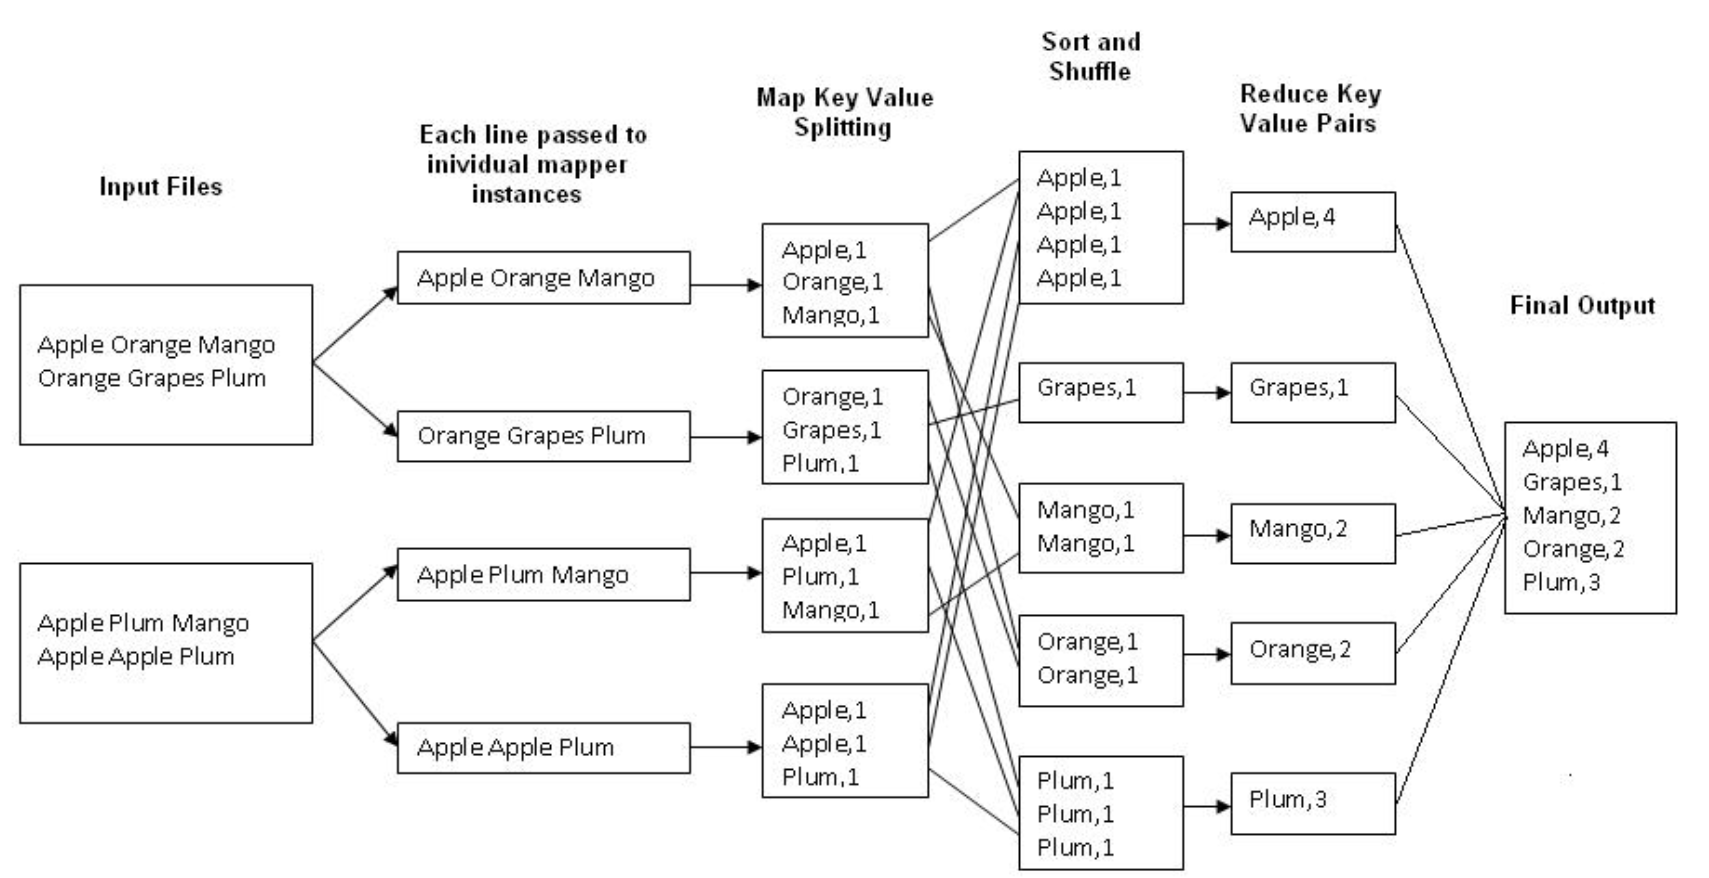
\includegraphics{images/14/hadoop_wordcount.png}
   \caption{Hadoop WordCount example, equivalent to \textit{Hello world!}}
   \label{fig:14/hadoop_wordcount}
\end{figure}
 In \autoref{fig:14/hadoop_wordcount} \textit{``individual mapper''} refers to a node implementing map.

In the slides there are some ---not complete--- instructions in Python to implement a simple WordCount using Hadoop.

\begin{lstlisting}[caption={Launching hadoop}]
   hadoop jar
   $HADOOP_HOME/share/hadoop/tools/lib/hadoop-
   streaming-*.jar \
   -input /user/hadoop/input \
   -output /user/hadoop/output \
   -mapper mapper.py \
   -reducer reducer.py \
   -file mapper.py \
   -file reducer.py
\end{lstlisting}

Hadoop has been the first widely used solution, but nowdays also other solutions exists, such as Spark, while Hadoop is considered somehow outdated.

\section{Spark}
\begin{paracol}{2}
   \begin{figure}[htbp]
      \centering
      
\includegraphics{images/14/spark_logo.png}
      \caption{Spark logo}
      \label{fig:14/spark_logo}
   \end{figure}
   \switchcolumn
   Spark is a fast and general-purpose cluster computing system. It provides high-level APIs in Java, Scala, Python, and R, and an optimized engine that supports general execution graphs. It also supports a rich set of higher-level tools including Spark SQL for SQL and structured data processing, MLlib for machine learning, GraphX for graph processing, and Spark Streaming (quite outdated, the updated version is \textit{``Spark structured streaming''}).
\end{paracol}

\framedt{Lazy vs Eager evalutation}{
   \begin{definition}
      \textbf{Lazy evaluation} is an evaluation strategy that delays the evaluation of an expression until its value is actually required (a dependent expression is evaluated).
   \end{definition}

   \begin{definition}
      \textbf{Eager evaluation} is an evaluation strategy that evaluates an expression as soon as it is bound to a variable.
   \end{definition}
}

\note{As we will see Spark is based on lazy evaluation, which allows to optimize the execution plan.
}

\subsection{Architecture}
Every Spark application consists of a \textit{driver} program running the \textit{main} function and executing various parallel operations on a cluster. The driver program accesses Spark through a \textit{SparkSession} object, which represents a connection to a Spark cluster.

\begin{paracol}{2}
   The main abstraction Spark provides is a \textbf{resilient distributed dataset} (\texttt{RDD}), which is a collection of elements partitioned across the nodes of the cluster that can be operated on in parallel.
   \begin{definition}
      [RDD]
      It \ul{is a single \textbf{immutable} distributed collection of objects}.\\
      Each dataset is divided into logical partitions, which may be computed on different nodes of the cluster.\\
      RDDs can contain any type of Python, Java, or Scala objects, including user-defined classes.
   \end{definition}
   
   \switchcolumn

   \begin{figure}[htbp]
      \centering
      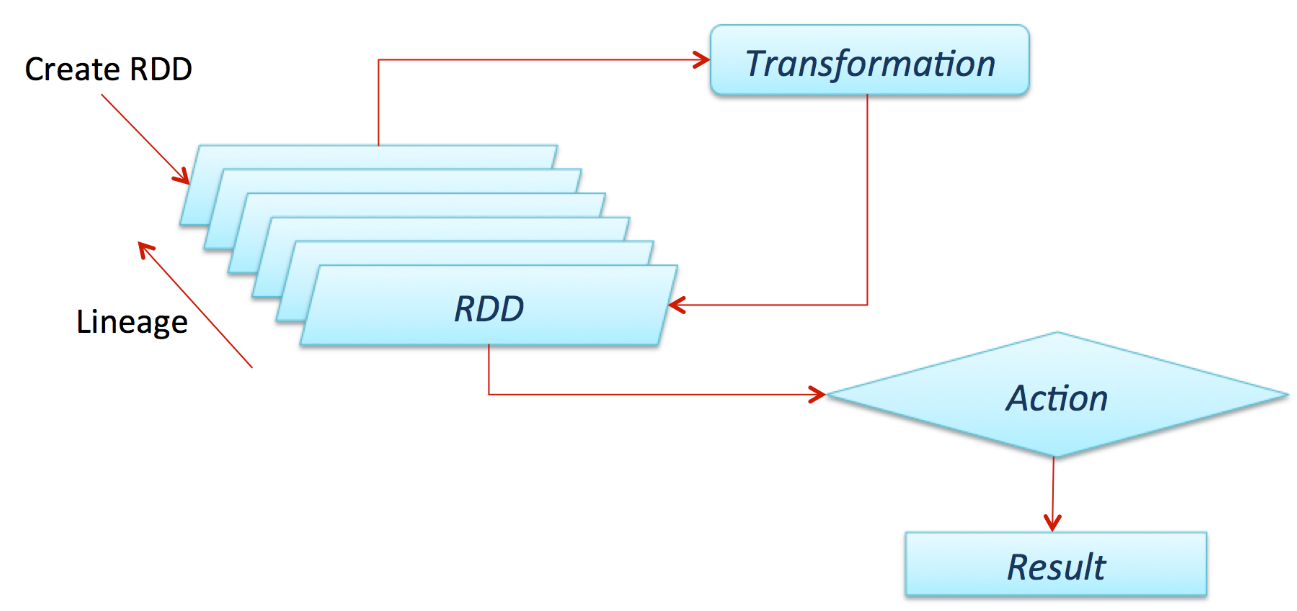
\includegraphics[width=0.9\columnwidth]{images/14/spark_rdd.png}
      \caption{RDD schema}
      \label{fig:14/spark_rdd}
   \end{figure}

\end{paracol}

\note{Note that since an RDD is a single \textit{immutable} distributed collection of objects, it fits nicely in the functional programming paradigm.}

\begin{paracol}{2}
   \begin{lstlisting}[language=Python, caption={Creating an RDD}]
      data = [1, 2, 3, 4, 5]
      distData = sc.parallelize(data)
      distFile = sc.textFile("data.txt")
   \end{lstlisting}
   \switchcolumn
   RDDs may be created by parallelizing an existing collection in your driver program, or by referencing an external dataset such as a shared file system, HDFS, HBase, or any data source offering a Hadoop InputFormat.
\end{paracol}
   
RDD can be persisted in memory, allowing it to be reused efficiently across parallel operations.
\ul{RDDs automatically recover from node failures}.
\note{RDDs can be created from Hadoop InputFormats (such as HDFS files) or by transforming other RDDs.}
\nl

Another abstraction in Spark are \textbf{shared variables}, which are \textbf{broadcast} variables and \textbf{accumulators}.\\
When Spark runs a function in parallel as a set of tasks on different nodes, it ships a copy of each variable used in the function to each task.
{A variable may need to be shared across tasks, or between tasks and the driver program. Spark supports two types of shared variables:\ns
\begin{itemize}
   \item \textbf{Broadcast variables} - allow the programmer to keep a read-only variable cached on each machine rather than shipping a copy of it with tasks.
   \item \textbf{Accumulators} - are variables that are only added to through an associative operation and can therefore be efficiently supported in parallel.
\end{itemize}}

{RDDs support two types of operations: \textbf{transformations} and \textbf{actions}.\ns
\begin{itemize}
   \item \textbf{Transformations} - create a new dataset from an existing one. These are \textit{lazy} operations, meaning that Spark doesn't apply the transformation immediately, but remembers the transformation applied to the base dataset.
   \item \textbf{Actions} - return a value to the driver program after running a computation on the dataset.
   When an action is called, Spark computes the result of the transformation chain.
\end{itemize}}

\begin{paracol}{2}
   \begin{lstlisting}
      lineLengths = lines.map(lambda s: len(s))
      totalLength = lineLengths.reduce(lambda a, b: a + b)
      # lineLengths gets consumed by the reduce
      # we can instruct Spark to persist the RDD
      # lineLengths.persist() # place before reduce

   \end{lstlisting}
   
   \switchcolumn

   \lstinline|lineLengths| holds the result of the \lstinline|map| \textbf{transformation}, which however is not computed instantaneously ---due to \textit{lazyness}---, and \lstinline|totalLength| holds the result of the \lstinline|reduce| \textbf{action}.
   At this point, 
   Spark breaks the computation into tasks to run on
   separate machines, and each machine runs both its part of the map and a local reduction, returning only its answer to the driver program.
\end{paracol}


Note that being RDDs immutable allows for three key advantages:
\begin{enumerate}
   \item \textbf{Consistency} - optimizations and lazy evaluation of transformations wouldn't be possible if the RDDs were mutable. 
   Besides, we can always go back to the original RDD, and there is no need to keep track of the changes and replicas of the data.
   \item \textbf{Resiliency} - if a node fails, the RDD can be recomputed from the original data.
   \item \textbf{Concurrency} - multiple tasks can operate on the same RDD without worrying about the data being changed, so zero concurrency issues.
\end{enumerate}


Implementing a simple WordCount in Spark is quite simple, as shown in \autoref{fig:14/spark_wordcount}.
This is much simpler than setting up hadoop.
\begin{lstlisting}[language=Python, caption={Spark WordCount example}]
   import sys
   from pyspark import SparkContext
   sc = SparkContext(appName="WordCountExample")
   lines = sc.textFile(sys.argv[1])
   counts = lines.flatMap(lambda x: x.split(' ')) \
      .map(lambda x: (x, 1)) \
      .reduceByKey(lambda x,y:x+y)
   output = counts.collect()
   for (word, count) in output:
      print "%s: %i" % (word, count)
   sc.stop()
\end{lstlisting}
